\documentclass[a4j,twoside,openright,11pt]{jarticle}
%
\usepackage{amsmath,amssymb}
\usepackage{bm}
\usepackage{graphicx}
\usepackage{ascmac}
\usepackage{listliketab}
\usepackage{url}
\usepackage{listings}

\setlength{\textwidth}{15.92cm}
\setlength{\oddsidemargin}{0mm}
\setlength{\evensidemargin}{0mm}
\setlength{\topmargin}{-1cm}
\setlength{\textheight}{23.5cm}
\setlength{\footskip}{18mm}

%
\pagestyle{plain}
\makeatletter
  \def\@maketitle{%
  \newpage\null
  \vskip 2em%
  \begin{center}%
  \let\footnote\thanks
    {\huge \@title \par}%
    \vskip 1.5em%
  \end{center}% 追加
  \begin{flushright}
        \@author
  \end{flushright}
  \begin{flushright}% 追加
    {\large \@date}%
  \end{flushright}%
  \par\vskip 1.5em}
\makeatother

\title{振動制御実験}
\author{九州工業大学 機械知能工学科 機械コース\\3年 学籍番号:13104069 坂本 悠作}
\date{
実験日1:平成27年6月17日\\
実験日2:平成27年6月24日\\
提出日 :平成27年6月30日
}
\begin{document}
\maketitle

\section{基本課題1}
授業内課題発表点 13
\newpage
\section{基本課題2}
\subsection{実験の感想}
機械工学実験の中では特に楽しめる内容であったと感じた。進行もスムーズに流れていたので、全体的に見れば良い実験であったと感じた。
\subsection{機械・宇宙システムの技術者として、制御をどう捉えるか}
現在の機械製品では、電子機器による制御が欠かせない状態にあるため、制御の知識・技術はある程度持っておくべきことであると考える。しかし、あまりにも電子制御に頼ってしまうと現代までに培われたからくり(例えば、ゼンマイで動作する機械式時計)のような技術を継承していく者は必要であると思う。
\subsection{PID制御とはなにか}
PID制御系の最も基本的な構成は図に示す通りである。
\begin{figure}[htbp]
\begin{center}
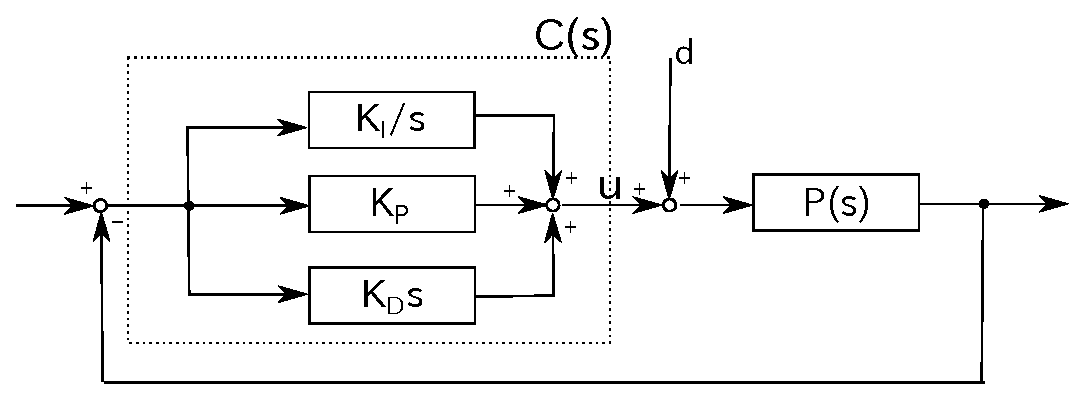
\includegraphics[width=12cm]{PID1.eps}
\end{center}
\caption{PID制御系の基本形}
\end{figure}
PID補償器$C(s)$は、比例・積分・微分の3つの要素を並列に結合したものである。$K_P,K_I,K_D$のパラメータは、それぞれ比例ゲイン・積分ゲイン・微分ゲインと呼ばれており、図1の$C(s)$をPID補償器と呼ぶ。このパラメータを決定するのには、主に限界感度法かステップ応答法が用いられる。限界感度法は持続振動をする比例パラメータ($u=K_ceのK_c$)を実験的に求め、Ziegler Nicholsによって提唱された調整方法でそれぞれのパラメータを求めていく。PID補償器の伝達関数を次式で示す。
\begin{eqnarray}
C(s)&=&K_P + K_I\frac{1}{s} + K_Ds\\
    &=&K_P(1+\frac{1}{T_Is}+T_Ds)
\end{eqnarray}
ここで、(2)式の$T_I \equiv \frac{K_P}{K_I},T_D \equiv \frac{K_D}{K_P}$である。$T_C$ = 振動周期とすると、Ziegler Nichols調整法によれば、表1のようになる。

\begin{table}[htb]
\begin{center}
  \caption{Ziegler Nichols調整法}
  \begin{tabular}{|l||c|c|c|} \hline
制御の種類&$K_P$     &積分時間$T_I$    &微分時間$T_D$\\
\hline
P        &0.50$K_u$ &-        &-\\
PI       &0.45$K_u$ &0.83$T_C$&-\\
PID      &0.60$K_u$ &0.50$T_C$&0.125$T_C$\\
\hline
  \end{tabular}
\end{center}
\end{table}

また、過渡応答法(ステップ応答法とも)によるパラメータ調整法では、制御対象単体にステップ状の入力を加えた時の応答から制御パラメータを求める。多くの場合はシグモイド曲線のような曲線となるので、曲線の最も急なところに接線を引き、その勾配をR,接線が時間軸と交わる時刻をLとすると、表2のようにパラメータを調整する。\begin{table}[htb]
\begin{center}
  \caption{過渡応答法}
  \begin{tabular}{|l||c|c|c|} \hline
制御の種類&$K_P$     &積分時間$T_I$    &微分時間$T_D$\\
\hline
P        &  1/RL &-        &-\\
PI       &0.9/RL &3.33L    &-\\
PID      &1.2/RL &2L       &0.5L\\
\hline
  \end{tabular}
\end{center}
\end{table}
このPID制御で全ての制御が行えるわけではなく、問題を起こすこともある。そのような場合は変形させて、D動作またはPD動作をフィードバックに移すことも有る。PD動作をフィードバックに移した形は比例・微分先行型PID制御またはI-PD制御と呼ばれる。
\par
どちらの調整法を適用してもオーバーシュートが発生してしまうので、必要であれば調整法を適用した後に微調整を行なう。
\subsection{最適制御とはなにか}
最適制御とは、制御系の設計における目標(ここでは、収束の速さ、入力の小ささ、変化の穏やかさ等を含む)を実現するために、重みに左右される評価関数(一般的には2次系式をとって負の値が出ないようにしている)を用意し、これを最小にするような制御系を設計する。欠点として、システム同定(入力と出力の関係を求めること)が難しいことや、多入力多出力多パラメータとなってしまうことが挙げられる。

\section{実験を改善する方策を述べよ}
\begin{enumerate}
\item 第1週目の倒立振子ロボットの組み立ては、目的が明確でなく時間の無駄だと感じましたのでロボットを事前に組み立てておくのがよろしいと思います。1週目2周目共に同じロボットを使用するのであれば、組み立て・分解する必要性が全く見当たりません。
\item 2周めの最適制御でのレースは必要ないと感じました。前週のPID制御でのレースとの違いが見当たらないので、もしも違いを明確に認識することが目的であったならば、違いが顕著に現れている動画等を撮影し、それを見比べる方が学習になったと思います。
\item 2周目の発表では、評価をする教員の方が完成度を求めすぎているように感じました。全員が誤解しないような言葉を使うように、という指摘ではなく、目的を絞って行なうほうがよろしいと思います。
\end{enumerate}
\section{最適制御よりもPID制御の方が非常に多くの場面で使われているのはなぜか}
ライントレースの走行制御を考えてみると、入力としてラインの位置とロボットの位置の距離を制御したい量、入力としてロボットの左右の車輪(モータ)の回転速度差を入力として与えると考える。このとき、ラインの片端をラインの位置として捉えるために、光センサ(参考文献1で用いられているような)ではなくカメラによる画像処理で目標値を取得すると仮定した。
\par
PID制御であれば、ラインとの距離に比例した比例制御、振動を抑えるための微分制御、標準偏差が無くなるために積分制御を入力量として算出する。限界感度法によってパラメータを決定する。最適制御であれば、ロボットが早くラインに近くなるように重みを重くする。
\par
最適制御は評価関数によってパラメータを求めることができるが、状態方程式によるモデリングが難しく、計算も難解であり、システム同定も困難である。対してPID制御では1入力1出力3パラメータであり、計算も簡単である。今考えているライントレースロボットは、車輪の回転数比を入力としてラインとロボットの距離を出力とする1入力1出力であるので、そこまで大変な計算ではなく、電圧値に比例してトルクが増加するようなDCモータを用いればシステム同定も簡単にできると予想される。PID制御でもかなり性能の良い制御が実現できるが(参考文献2の動画参照)、振動を起こさずにライン端に素早く収束する方が望ましいと考える。従ってこのライントレースロボットでは、最適制御をするほうが良いと考えた。

\section{参考文献}
\begin{enumerate}
\item \url{http://www.seto.nanzan-u.ac.jp/st/gr-thesis/ms/2011/08mi200.pdf}
\item \url{http://monoist.atmarkit.co.jp/mn/articles/1007/26/news083_2.html}
\item 機械工学実験2 実験書
\item はじめての現代制御理論 佐藤和也ら 講義14「最適制御」
\end{enumerate}

\end{document}
